

\tikzset{every picture/.style={line width=0.75pt}} %set default line width to 0.75pt        

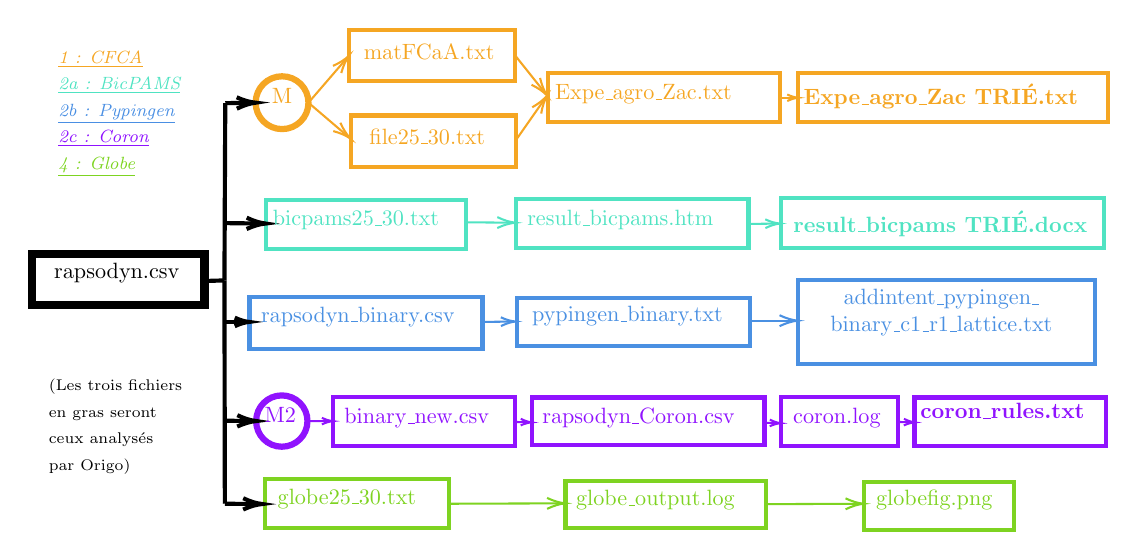
\begin{tikzpicture}[x=0.75pt,y=0.75pt,yscale=-.8,xscale=.8]
%uncomment if require: \path (0,365); %set diagram left start at 0, and has height of 365

%Shape: Rectangle [id:dp5112889087468507] 
\draw  [line width=3]  (7.57,160.08) -- (111.57,160.08) -- (111.57,191.08) -- (7.57,191.08) -- cycle ;
%Shape: Rectangle [id:dp34677739092923077] 
\draw  [color={rgb, 255:red, 245; green, 166; blue, 35 }  ,draw opacity=1 ][line width=1.5]  (198.57,25.12) -- (298.33,25.12) -- (298.33,56.12) -- (198.57,56.12) -- cycle ;
%Shape: Circle [id:dp09366737090816712] 
\draw  [color={rgb, 255:red, 245; green, 166; blue, 35 }  ,draw opacity=1 ][line width=2.25]  (142.37,69.05) .. controls (142.37,60.27) and (149.49,53.15) .. (158.27,53.15) .. controls (167.05,53.15) and (174.17,60.27) .. (174.17,69.05) .. controls (174.17,77.83) and (167.05,84.95) .. (158.27,84.95) .. controls (149.49,84.95) and (142.37,77.83) .. (142.37,69.05) -- cycle ;
%Shape: Circle [id:dp33523948187015884] 
\draw  [color={rgb, 255:red, 144; green, 19; blue, 254 }  ,draw opacity=1 ][line width=2.25]  (142.67,260.78) .. controls (142.67,252.25) and (149.58,245.33) .. (158.12,245.33) .. controls (166.65,245.33) and (173.57,252.25) .. (173.57,260.78) .. controls (173.57,269.32) and (166.65,276.23) .. (158.12,276.23) .. controls (149.58,276.23) and (142.67,269.32) .. (142.67,260.78) -- cycle ;
%Shape: Rectangle [id:dp07102445158620008] 
\draw  [color={rgb, 255:red, 245; green, 166; blue, 35 }  ,draw opacity=1 ][line width=1.5]  (199.67,76.72) -- (299.23,76.72) -- (299.23,107.72) -- (199.67,107.72) -- cycle ;
%Shape: Rectangle [id:dp3321678459396359] 
\draw  [color={rgb, 255:red, 245; green, 166; blue, 35 }  ,draw opacity=1 ][line width=1.5]  (318.23,51.08) -- (457.9,51.08) -- (457.9,80.75) -- (318.23,80.75) -- cycle ;
%Shape: Rectangle [id:dp5334183380754819] 
\draw  [color={rgb, 255:red, 245; green, 166; blue, 35 }  ,draw opacity=1 ][line width=1.5]  (469.03,51.42) -- (655.43,51.42) -- (655.43,80.68) -- (469.03,80.68) -- cycle ;
%Shape: Rectangle [id:dp4003910061407878] 
\draw  [color={rgb, 255:red, 80; green, 227; blue, 194 }  ,draw opacity=1 ][line width=1.5]  (458.73,126.42) -- (653.48,126.42) -- (653.48,156.67) -- (458.73,156.67) -- cycle ;
%Shape: Rectangle [id:dp8380864565956413] 
\draw  [color={rgb, 255:red, 80; green, 227; blue, 194 }  ,draw opacity=1 ][line width=1.5]  (299.2,127) -- (439.15,127) -- (439.15,156.5) -- (299.2,156.5) -- cycle ;
%Shape: Rectangle [id:dp6634021266628283] 
\draw  [color={rgb, 255:red, 80; green, 227; blue, 194 }  ,draw opacity=1 ][line width=1.5]  (148.83,127.5) -- (269.23,127.5) -- (269.23,157) -- (148.83,157) -- cycle ;
%Shape: Rectangle [id:dp09471322366323875] 
\draw  [color={rgb, 255:red, 74; green, 144; blue, 226 }  ,draw opacity=1 ][line width=1.5]  (138.62,186.23) -- (279.02,186.23) -- (279.02,217.23) -- (138.62,217.23) -- cycle ;
%Shape: Rectangle [id:dp357448816640074] 
\draw  [color={rgb, 255:red, 74; green, 144; blue, 226 }  ,draw opacity=1 ][line width=1.5]  (299.52,186.58) -- (439.92,186.58) -- (439.92,215.43) -- (299.52,215.43) -- cycle ;
%Shape: Rectangle [id:dp4037996924419438] 
\draw  [color={rgb, 255:red, 74; green, 144; blue, 226 }  ,draw opacity=1 ][line width=1.5]  (468.82,226.42) -- (648.07,226.42) -- (648.07,176.08) -- (468.82,176.08) -- cycle ;
%Shape: Rectangle [id:dp006682035621268012] 
\draw  [color={rgb, 255:red, 144; green, 19; blue, 254 }  ,draw opacity=1 ][line width=1.5]  (188.82,246.33) -- (298.47,246.33) -- (298.47,275.58) -- (188.82,275.58) -- cycle ;
%Shape: Rectangle [id:dp2670592101040946] 
\draw  [color={rgb, 255:red, 144; green, 19; blue, 254 }  ,draw opacity=1 ][line width=1.5]  (308.57,246.58) -- (448.82,246.58) -- (448.82,275.33) -- (308.57,275.33) -- cycle ;
%Shape: Rectangle [id:dp25697946311686126] 
\draw  [color={rgb, 255:red, 144; green, 19; blue, 254 }  ,draw opacity=1 ][line width=1.5]  (458.57,246.08) -- (529.02,246.08) -- (529.02,275.58) -- (458.57,275.58) -- cycle ;
%Shape: Rectangle [id:dp9512931041854022] 
\draw  [color={rgb, 255:red, 144; green, 19; blue, 254 }  ,draw opacity=1 ][line width=1.5]  (539.17,246.58) -- (654.37,246.58) -- (654.37,275.83) -- (539.17,275.83) -- cycle ;
%Shape: Rectangle [id:dp6785275622055427] 
\draw  [color={rgb, 255:red, 126; green, 211; blue, 33 }  ,draw opacity=1 ][line width=1.5]  (147.9,295.68) -- (258.57,295.68) -- (258.57,325.33) -- (147.9,325.33) -- cycle ;
%Shape: Rectangle [id:dp6714296332776397] 
\draw  [color={rgb, 255:red, 126; green, 211; blue, 33 }  ,draw opacity=1 ][line width=1.5]  (328.93,296.85) -- (449.57,296.85) -- (449.57,325.42) -- (328.93,325.42) -- cycle ;
%Shape: Rectangle [id:dp7840710281848223] 
\draw  [color={rgb, 255:red, 126; green, 211; blue, 33 }  ,draw opacity=1 ][line width=1.5]  (508.67,297.33) -- (599.07,297.33) -- (599.07,326.28) -- (508.67,326.28) -- cycle ;
%Straight Lines [id:da10768594729227787] 
\draw [color={rgb, 255:red, 245; green, 166; blue, 35 }  ,draw opacity=1 ]   (174.17,69.05) -- (197.26,42.26) ;
\draw [shift={(198.57,40.75)}, rotate = 130.77] [color={rgb, 255:red, 245; green, 166; blue, 35 }  ,draw opacity=1 ][line width=0.75]    (10.93,-3.29) .. controls (6.95,-1.4) and (3.31,-0.3) .. (0,0) .. controls (3.31,0.3) and (6.95,1.4) .. (10.93,3.29)   ;
%Straight Lines [id:da8200270235520359] 
\draw [color={rgb, 255:red, 245; green, 166; blue, 35 }  ,draw opacity=1 ]   (174.17,69.05) -- (198.05,89.45) ;
\draw [shift={(199.57,90.75)}, rotate = 220.51] [color={rgb, 255:red, 245; green, 166; blue, 35 }  ,draw opacity=1 ][line width=0.75]    (10.93,-3.29) .. controls (6.95,-1.4) and (3.31,-0.3) .. (0,0) .. controls (3.31,0.3) and (6.95,1.4) .. (10.93,3.29)   ;
%Straight Lines [id:da6724334215432369] 
\draw [color={rgb, 255:red, 245; green, 166; blue, 35 }  ,draw opacity=1 ]   (299.23,91.42) -- (316.75,66.39) ;
\draw [shift={(317.9,64.75)}, rotate = 124.99] [color={rgb, 255:red, 245; green, 166; blue, 35 }  ,draw opacity=1 ][line width=0.75]    (10.93,-3.29) .. controls (6.95,-1.4) and (3.31,-0.3) .. (0,0) .. controls (3.31,0.3) and (6.95,1.4) .. (10.93,3.29)   ;
%Straight Lines [id:da09608921555621242] 
\draw [color={rgb, 255:red, 245; green, 166; blue, 35 }  ,draw opacity=1 ]   (298.23,40.08) -- (316.65,63.19) ;
\draw [shift={(317.9,64.75)}, rotate = 231.43] [color={rgb, 255:red, 245; green, 166; blue, 35 }  ,draw opacity=1 ][line width=0.75]    (10.93,-3.29) .. controls (6.95,-1.4) and (3.31,-0.3) .. (0,0) .. controls (3.31,0.3) and (6.95,1.4) .. (10.93,3.29)   ;
%Straight Lines [id:da7881183362280086] 
\draw [color={rgb, 255:red, 245; green, 166; blue, 35 }  ,draw opacity=1 ]   (457.82,66.08) -- (467.07,66.08) ;
\draw [shift={(469.07,66.08)}, rotate = 180] [color={rgb, 255:red, 245; green, 166; blue, 35 }  ,draw opacity=1 ][line width=0.75]    (6.56,-1.97) .. controls (4.17,-0.84) and (1.99,-0.18) .. (0,0) .. controls (1.99,0.18) and (4.17,0.84) .. (6.56,1.97)   ;
%Straight Lines [id:da9573949983682682] 
\draw [color={rgb, 255:red, 80; green, 227; blue, 194 }  ,draw opacity=1 ]   (438.82,142.08) -- (456.07,141.86) ;
\draw [shift={(458.07,141.83)}, rotate = 179.26] [color={rgb, 255:red, 80; green, 227; blue, 194 }  ,draw opacity=1 ][line width=0.75]    (8.74,-2.63) .. controls (5.56,-1.12) and (2.65,-0.24) .. (0,0) .. controls (2.65,0.24) and (5.56,1.12) .. (8.74,2.63)   ;
%Straight Lines [id:da19856323362407713] 
\draw [color={rgb, 255:red, 80; green, 227; blue, 194 }  ,draw opacity=1 ]   (269.57,141.08) -- (296.82,141.32) ;
\draw [shift={(298.82,141.33)}, rotate = 180.49] [color={rgb, 255:red, 80; green, 227; blue, 194 }  ,draw opacity=1 ][line width=0.75]    (10.93,-3.29) .. controls (6.95,-1.4) and (3.31,-0.3) .. (0,0) .. controls (3.31,0.3) and (6.95,1.4) .. (10.93,3.29)   ;
%Straight Lines [id:da3882843389789006] 
\draw [color={rgb, 255:red, 74; green, 144; blue, 226 }  ,draw opacity=1 ]   (279.57,201.08) -- (296.82,200.86) ;
\draw [shift={(298.82,200.83)}, rotate = 179.26] [color={rgb, 255:red, 74; green, 144; blue, 226 }  ,draw opacity=1 ][line width=0.75]    (8.74,-2.63) .. controls (5.56,-1.12) and (2.65,-0.24) .. (0,0) .. controls (2.65,0.24) and (5.56,1.12) .. (8.74,2.63)   ;
%Straight Lines [id:da31466226163875344] 
\draw [color={rgb, 255:red, 74; green, 144; blue, 226 }  ,draw opacity=1 ]   (440.07,200.33) -- (466.82,200.33) ;
\draw [shift={(468.82,200.33)}, rotate = 180] [color={rgb, 255:red, 74; green, 144; blue, 226 }  ,draw opacity=1 ][line width=0.75]    (10.93,-3.29) .. controls (6.95,-1.4) and (3.31,-0.3) .. (0,0) .. controls (3.31,0.3) and (6.95,1.4) .. (10.93,3.29)   ;
%Straight Lines [id:da8134370105916718] 
\draw [color={rgb, 255:red, 144; green, 19; blue, 254 }  ,draw opacity=1 ]   (448.82,261.83) -- (456.57,262.03) ;
\draw [shift={(458.57,262.08)}, rotate = 181.47] [color={rgb, 255:red, 144; green, 19; blue, 254 }  ,draw opacity=1 ][line width=0.75]    (6.56,-1.97) .. controls (4.17,-0.84) and (1.99,-0.18) .. (0,0) .. controls (1.99,0.18) and (4.17,0.84) .. (6.56,1.97)   ;
%Straight Lines [id:da6276850519992108] 
\draw [color={rgb, 255:red, 144; green, 19; blue, 254 }  ,draw opacity=1 ]   (298.82,261.33) -- (306.57,261.53) ;
\draw [shift={(308.57,261.58)}, rotate = 181.47] [color={rgb, 255:red, 144; green, 19; blue, 254 }  ,draw opacity=1 ][line width=0.75]    (6.56,-1.97) .. controls (4.17,-0.84) and (1.99,-0.18) .. (0,0) .. controls (1.99,0.18) and (4.17,0.84) .. (6.56,1.97)   ;
%Straight Lines [id:da10203542644843089] 
\draw [color={rgb, 255:red, 144; green, 19; blue, 254 }  ,draw opacity=1 ]   (173.57,260.78) -- (186.82,260.83) ;
\draw [shift={(188.82,260.83)}, rotate = 180.19] [color={rgb, 255:red, 144; green, 19; blue, 254 }  ,draw opacity=1 ][line width=0.75]    (6.56,-1.97) .. controls (4.17,-0.84) and (1.99,-0.18) .. (0,0) .. controls (1.99,0.18) and (4.17,0.84) .. (6.56,1.97)   ;
%Straight Lines [id:da4429224871441608] 
\draw [color={rgb, 255:red, 126; green, 211; blue, 33 }  ,draw opacity=1 ]   (258.82,310.58) -- (326.82,310.34) ;
\draw [shift={(328.82,310.33)}, rotate = 179.8] [color={rgb, 255:red, 126; green, 211; blue, 33 }  ,draw opacity=1 ][line width=0.75]    (10.93,-3.29) .. controls (6.95,-1.4) and (3.31,-0.3) .. (0,0) .. controls (3.31,0.3) and (6.95,1.4) .. (10.93,3.29)   ;
%Straight Lines [id:da03639386162212155] 
\draw [color={rgb, 255:red, 126; green, 211; blue, 33 }  ,draw opacity=1 ]   (449.82,310.83) -- (506.57,310.59) ;
\draw [shift={(508.57,310.58)}, rotate = 179.76] [color={rgb, 255:red, 126; green, 211; blue, 33 }  ,draw opacity=1 ][line width=0.75]    (10.93,-3.29) .. controls (6.95,-1.4) and (3.31,-0.3) .. (0,0) .. controls (3.31,0.3) and (6.95,1.4) .. (10.93,3.29)   ;
%Straight Lines [id:da4808508336370918] 
\draw [color={rgb, 255:red, 144; green, 19; blue, 254 }  ,draw opacity=1 ]   (529.57,261.33) -- (537.32,261.53) ;
\draw [shift={(539.32,261.58)}, rotate = 181.47] [color={rgb, 255:red, 144; green, 19; blue, 254 }  ,draw opacity=1 ][line width=0.75]    (6.56,-1.97) .. controls (4.17,-0.84) and (1.99,-0.18) .. (0,0) .. controls (1.99,0.18) and (4.17,0.84) .. (6.56,1.97)   ;
%Straight Lines [id:da7722405754500837] 
\draw [line width=1.5]    (111.9,176.42) -- (123.57,176.08) ;
%Straight Lines [id:da7091724677313925] 
\draw [line width=1.5]    (124.07,69.33) -- (123.57,176.08) ;
%Straight Lines [id:da3934697170079686] 
\draw [line width=1.5]    (123.57,176.08) -- (123.82,310.58) ;
%Straight Lines [id:da6551167134439269] 
\draw [line width=1.5]    (123.82,310.58) -- (143.23,310.73) ;
\draw [shift={(146.23,310.75)}, rotate = 180.43] [color={rgb, 255:red, 0; green, 0; blue, 0 }  ][line width=1.5]    (11.37,-3.42) .. controls (7.23,-1.45) and (3.44,-0.31) .. (0,0) .. controls (3.44,0.31) and (7.23,1.45) .. (11.37,3.42)   ;
%Straight Lines [id:da10063747529252298] 
\draw [line width=1.5]    (123.82,260.58) -- (139.67,260.75) ;
\draw [shift={(142.67,260.78)}, rotate = 180.61] [color={rgb, 255:red, 0; green, 0; blue, 0 }  ][line width=1.5]    (11.37,-3.42) .. controls (7.23,-1.45) and (3.44,-0.31) .. (0,0) .. controls (3.44,0.31) and (7.23,1.45) .. (11.37,3.42)   ;
%Straight Lines [id:da20539738841469357] 
\draw [line width=1.5]    (123.57,201.08) -- (135.32,201.08) ;
\draw [shift={(138.32,201.08)}, rotate = 180] [color={rgb, 255:red, 0; green, 0; blue, 0 }  ][line width=1.5]    (8.53,-2.57) .. controls (5.42,-1.09) and (2.58,-0.23) .. (0,0) .. controls (2.58,0.23) and (5.42,1.09) .. (8.53,2.57)   ;
%Straight Lines [id:da44318693870092873] 
\draw [line width=1.5]    (124.07,141.58) -- (145.32,141.8) ;
\draw [shift={(148.32,141.83)}, rotate = 180.59] [color={rgb, 255:red, 0; green, 0; blue, 0 }  ][line width=1.5]    (11.37,-3.42) .. controls (7.23,-1.45) and (3.44,-0.31) .. (0,0) .. controls (3.44,0.31) and (7.23,1.45) .. (11.37,3.42)   ;
%Straight Lines [id:da9403767790329779] 
\draw [line width=1.5]    (124.07,69.33) -- (139.37,69.1) ;
\draw [shift={(142.37,69.05)}, rotate = 179.11] [color={rgb, 255:red, 0; green, 0; blue, 0 }  ][line width=1.5]    (11.37,-3.42) .. controls (7.23,-1.45) and (3.44,-0.31) .. (0,0) .. controls (3.44,0.31) and (7.23,1.45) .. (11.37,3.42)   ;

% Text Node
\draw (19.57,164.08) node [anchor=north west][inner sep=0.75pt] [xscale=0.8,yscale=0.8] [align=left] {rapsodyn.csv};
% Text Node
\draw (150.57,58.75) node [anchor=north west][inner sep=0.75pt]  [color={rgb, 255:red, 245; green, 166; blue, 35 }  ,opacity=1 ,xscale=0.8,yscale=0.8] [align=left] {M};
% Text Node
\draw (206,32.38) node [anchor=north west][inner sep=0.75pt]  [color={rgb, 255:red, 245; green, 166; blue, 35 }  ,opacity=1 ,xscale=0.8,yscale=0.8] [align=left] {matFCaA.txt};
% Text Node
\draw (209.42,83.38) node [anchor=north west][inner sep=0.75pt]  [color={rgb, 255:red, 245; green, 166; blue, 35 }  ,opacity=1 ,xscale=0.8,yscale=0.8] [align=left] {file25\_30.txt};
% Text Node
\draw (321.17,56.75) node [anchor=north west][inner sep=0.75pt]  [color={rgb, 255:red, 245; green, 166; blue, 35 }  ,opacity=1 ,xscale=0.8,yscale=0.8] [align=left] {Expe\_agro\_Zac.txt};
% Text Node
\draw (470.83,56.22) node [anchor=north west][inner sep=0.75pt]  [color={rgb, 255:red, 245; green, 166; blue, 35 }  ,opacity=1 ,xscale=0.8,yscale=0.8] [align=left] {\textbf{Expe\_agro\_Zac TRIÉ.txt}};
% Text Node
\draw (151.23,132.5) node [anchor=north west][inner sep=0.75pt]  [color={rgb, 255:red, 80; green, 227; blue, 194 }  ,opacity=1 ,xscale=0.8,yscale=0.8] [align=left] {bicpams25\_30.txt};
% Text Node
\draw (304.48,132.5) node [anchor=north west][inner sep=0.75pt]  [color={rgb, 255:red, 80; green, 227; blue, 194 }  ,opacity=1 ,xscale=0.8,yscale=0.8] [align=left] {result\_bicpams.htm};
% Text Node
\draw (464.73,133.05) node [anchor=north west][inner sep=0.75pt]  [color={rgb, 255:red, 80; green, 227; blue, 194 }  ,opacity=1 ,xscale=0.8,yscale=0.8] [align=left] {\textbf{result\_bicpams TRIÉ.docx}};
% Text Node
\draw (144.12,190.58) node [anchor=north west][inner sep=0.75pt]  [color={rgb, 255:red, 74; green, 144; blue, 226 }  ,opacity=1 ,xscale=0.8,yscale=0.8] [align=left] {rapsodyn\_binary.csv};
% Text Node
\draw (307.37,190.33) node [anchor=north west][inner sep=0.75pt]  [color={rgb, 255:red, 74; green, 144; blue, 226 }  ,opacity=1 ,xscale=0.8,yscale=0.8] [align=left] {pypingen\_binary.txt};
% Text Node
\draw (479.37,180.08) node [anchor=north west][inner sep=0.75pt]  [color={rgb, 255:red, 74; green, 144; blue, 226 }  ,opacity=1 ,xscale=0.8,yscale=0.8] [align=left] {\begin{minipage}[lt]{111.63pt}\setlength\topsep{0pt}
\begin{center}
addintent\_pypingen\_\\binary\_c1\_r1\_lattice.txt
\end{center}

\end{minipage}};
% Text Node
\draw (146.32,251.33) node [anchor=north west][inner sep=0.75pt]  [color={rgb, 255:red, 144; green, 19; blue, 254 }  ,opacity=1 ,xscale=0.8,yscale=0.8] [align=left] {{\selectfont M2}};
% Text Node
\draw (194.32,251.58) node [anchor=north west][inner sep=0.75pt]  [color={rgb, 255:red, 144; green, 19; blue, 254 }  ,opacity=1 ,xscale=0.8,yscale=0.8] [align=left] {binary\_new.csv};
% Text Node
\draw (313.57,251.58) node [anchor=north west][inner sep=0.75pt]  [color={rgb, 255:red, 144; green, 19; blue, 254 }  ,opacity=1 ,xscale=0.8,yscale=0.8] [align=left] {rapsodyn\_Coron.csv};
% Text Node
\draw (464.62,251.33) node [anchor=north west][inner sep=0.75pt]  [color={rgb, 255:red, 144; green, 19; blue, 254 }  ,opacity=1 ,xscale=0.8,yscale=0.8] [align=left] {coron.log};
% Text Node
\draw (541.17,248.68) node [anchor=north west][inner sep=0.75pt]  [color={rgb, 255:red, 144; green, 19; blue, 254 }  ,opacity=1 ,xscale=0.8,yscale=0.8] [align=left] {\textbf{coron\_rules.txt}};
% Text Node
\draw (154.15,300) node [anchor=north west][inner sep=0.75pt]  [color={rgb, 255:red, 126; green, 211; blue, 33 }  ,opacity=1 ,xscale=0.8,yscale=0.8] [align=left] {globe25\_30.txt};
% Text Node
\draw (333.9,301) node [anchor=north west][inner sep=0.75pt]  [color={rgb, 255:red, 126; green, 211; blue, 33 }  ,opacity=1 ,xscale=0.8,yscale=0.8] [align=left] {globe\_output.log};
% Text Node
\draw (514.57,300.83) node [anchor=north west][inner sep=0.75pt]  [color={rgb, 255:red, 126; green, 211; blue, 33 }  ,opacity=1 ,xscale=0.8,yscale=0.8] [align=left] {globefig.png};

% Text Node
\draw (22,36.38) node [anchor=north west][inner sep=0.75pt]  [color={rgb, 255:red, 245; green, 166; blue, 35 }  ,opacity=1 ,xscale=0.8,yscale=0.8] [align=left] {\textit{{\footnotesize \underline{1 : CFCA}}}\\\textcolor[rgb]{0.31,0.89,0.76}{\textit{{\footnotesize \underline{2a : BicPAMS}}}}\\\textcolor[rgb]{0.29,0.56,0.89}{\textit{{\footnotesize \underline{2b : Pypingen}}}}\\\textcolor[rgb]{0.56,0.07,1}{\textit{{\footnotesize \underline{2c : Coron}}}}\\\textcolor[rgb]{0.49,0.83,0.13}{\textit{{\footnotesize \underline{4 : Globe}}}}};

% Text Node
\draw (16.33,234) node [anchor=north west][inner sep=0.75pt]  [xscale=0.8,yscale=0.8] [align=left] {{\scriptsize \textit{{\fontfamily{helvet}\selectfont (Les trois fichiers}}}\\{\scriptsize \textit{{\fontfamily{helvet}\selectfont en gras seront}}}\\{\scriptsize \textit{{\fontfamily{helvet}\selectfont ceux analysés}}}\\{\scriptsize \textit{{\fontfamily{helvet}\selectfont par Origo)}}}};



\end{tikzpicture}
